\onecolumn

\counterwithin{theorem}{section}
\counterwithin{lemma}{section}
\counterwithin{corollary}{section}
\counterwithin{definition}{section}
\counterwithin{example}{section}

\section{Extended Theoretical Characterization and Proofs} \label{sec:proofs-appendix}
We provide proofs for supplemental results and intermediary theorems used to derive or expand on our main theorems. \Cref{sec:properties-appendix} introduces some additional properties and terms used in the literature that we utilize in our full proofs; \Cref{sec:property-lemmas} through \Cref{sec:d-unstable-appendix} elaborate on instability, culminating in \Cref{sec:instability-proof} where we explicitly connect the proof of \Cref{thm:instability} to the contents of the prior subsections. Similarly, \Cref{sec:variability-appendix} through \Cref{sec:high-variability-appendix} focus on variability, and \Cref{sec:variability-proof} proves \Cref{thm:variability} using the the previously established theorems. Lastly, we conclude this appendix section with \Cref{sec:ml-prop-proof}, where we prove \Cref{prop:ml-representation}, and \Cref{sec:program-prop-proof}, where we prove \Cref{prop:program-variability}.

\subsection{Additional, Existing Choice Function Properties}\label{sec:properties-appendix}
In addition to \Cref{def:q-acceptance} and \Cref{def:substitutability}, which we restate here, we introduce several additional properties, and provide plain English intuition for all of them:

\qacceptance*
\textit{Intuition}: Capacity of $q$.

\substitutability*
\textit{Intuition}: Students selected from a larger pool remain selected when the pool shrinks.

\begin{restatable}[Monotonicity]{definition}{monotonicity}
\label{def:monotonicity}
Choice function $\choice$ is \textit{monotonic} if $X_1 \subseteq X_2$ implies $\choice(X_1) \subseteq \choice(X_2)$.
\end{restatable}
\textit{Intuition}: Students selected from a smaller pool remain selected when the pool expands.

\textbf{Note:} Monotonicity is much less studied than substitutability, but is conceptually and mathematically useful to understand as an ``inverse'' of substitutability.

\begin{restatable}[Consistency]{definition}{consistency}
\label{def:consistency}
Choice function $\choice$ is \textit{consistent} if $\choice(X_2) \subseteq X_1 \subseteq X_2$ implies $\choice(X_2) = \choice(X_1)$.
\end{restatable}
\textit{Intuition}: Removing rejected candidates from the input does not change the output.

\textbf{Note:} This is equivalent to the Independence of Irrelevant Alternatives, a common assumption in preference models, over elements. Note that this is distinct from substitutability; there exist inconsistent substitutable functions, and non-substitutable consistent functions. %

\begin{restatable}[$q$-representativeness]{definition}{qrepresentativeness}
\label{def:q-representative}
$q$-acceptant choice function $\choice$ is $q$-representative if there exists a strict total ordering $\succ$ over all $x \in \calX$ and $\choice(X)$ is the top $q$ elements of $X$ for all $X \subseteq \calX$.
\end{restatable}

\textit{Intuition}: Students are selected according to an exact ranking.

\textbf{Note:} We refer to this property in the main body as being ``characterized by a total order'', or a ``queue'', but this language --- and definition as a property in its own right --- is seen in, e.g., \citet{echenique2015control}.

\subsection{Property Lemmas}\label{sec:property-lemmas}

We introduce some quick lemmas about the above properties that simplify the proofs of our main results.

\paragraph{Fundamental Incompatibility}

A key structural constraint emerges immediately between monotonicity and $q$-acceptance.

\begin{restatable}[Incompatibility of Monotonicity and $q$-Acceptance]{lemma}{incompatibility}
\label{thm:mono-accept-mutex}
For $|\calX| > q \geq 1$, no choice function can be both monotonic and $q$-acceptant.
\end{restatable}

\textit{Intuition}: %
For a choice function to be monotonic, it must never reject a previously accepted applicant as the applicant pool grows. This implies that the capacity must be unbounded, which contradicts the strict capacity limit imposed by $q$-acceptance.%

\begin{proof}
Consider two different sets each of $q$ elements. If $\choice$ is $q$-acceptant, every element must be chosen in each. Then consider their union. If $\choice$ is monotonic, every element in their union would also be accepted, but that would contradict the $q$-acceptant capacity constraint.

Consider two disjoint sets $X_1, X_2 \subseteq \calX$ with $|X_1| = |X_2| = q$. By $q$-acceptance, $\choice(X_1) = X_1$ and $\choice(X_2) = X_2$. By monotonicity, both $\choice(X_1)$ and $\choice(X_2)$ must be subsets of $\choice(X_1 \cup X_2)$. But then $|\choice(X_1 \cup X_2)| \geq |X_1| + |X_2| = 2q > q$, violating $q$-acceptance.
\end{proof}

\paragraph{Non-Substitutable Functions}
\begin{restatable}{lemma}{unsubstitutable}
\label{lem:unsubstitutable}
If $\choice$ is not substitutable, there exists some $x^*$, $x'$, $X$ and $X' = X \cup \{x'\}$ where $x^* \in X$ and $x^* \in \choice(X')$ but $x^* \not\in \choice(X)$.
\end{restatable}

\textit{Intuition}:
If a choice function is not substitutable, then there is at least one situation where a decision ``flips'' from rejection to acceptance.
We argue that there has to be some single element $x'$ that causes this ``flip'' when added.

\begin{proof}
$\choice$ is not substitutable if there exists some  $x^*$ and $X_0 \subseteq X_k$ where $x^* \in X_0$ and $x^* \in \choice(X_k)$ but $x \not\in \choice(X_0)$.
Let $k$ be such that $k = |X_k \setminus X_0|$.%

We want to show the existence of $x'$. To do this, we identify the ``closest'' sets where this occurs. For each $x \in X_k \setminus X_0$, add elements to $X_0$, constructing $X_0 \subseteq X_1 \subseteq ... \subseteq X_j \subseteq ... \subseteq X_k$, where $X_1 = X_0 \cup \{x_1\}$ and so on. Let $X_j$ be the first in this sequence of sets such that $x^* \in \choice(X_j)$ where $x^* \in \choice(X_j)$ but $x^* \not\in \choice(X_{j-1})$. Then let $x' = x_j$, $X = X_{j-1}$, and $X' = X_j$.
\end{proof}

\subsection{Choice Distance} \label{sec:dist-appendix}

We provide some lemmas and a theorem about $r_\choice$,  defined in \Cref{def:distance}.

\begin{restatable}[Substitutability Term]{lemma}{sub-dist}
\label{lem:substitutability-term}
Choice function $\choice$ is substitutable if and only if $|X_1 \cap \choice(X_2) \setminus \choice(X_1)| = 0$ for all $X_1 \subseteq X_2$.
\end{restatable}

\textit{Intuition}:
For a substitutable choice function, previously rejected candidates are never accepted after the addition of more applicants. Thus labels cannot flip from negative to positive, which is what the first term counts.

\begin{proof}
For any sets $A, B$, $|A \setminus B| = 0$ if and only if $A \setminus B = \emptyset$, and furthermore $A \setminus B = \emptyset$ if and only if $A \subseteq B$. So $|X_1 \cap \choice(X_2) \setminus \choice(X_1)| = 0$ if and only if $X_1 \cap \choice(X_2) \subseteq \choice(X_1)$, which is the definition of substitutability.
\end{proof}

\begin{restatable}[Monotonicity Term]{lemma}{mono-dist}
\label{lem:monotonicity-term}
Choice function $\choice$ is monotonic if and only if $|\choice(X_1) \setminus \choice(X_2)| = 0$ for all $X_1 \subseteq X_2$.
\end{restatable}

\textit{Intuition}:
For a monotonic choice function, previously accepted candidates are never rejected after the addition of more applicants. Thus labels cannot flip from positive to negative, which is what the second term counts.

\begin{proof}
Use the same set properties as per \Cref{lem:substitutability-term},  $|\choice(X_1) \setminus \choice(X_2)| = 0$ if and only if $\choice(X_1) \subseteq \choice(X_2)$, which is the definition of monotonicity.
\end{proof}

\begin{restatable}[Triangle Inequality]{theorem}{triangle}
\label{thm:triangle-ineq}
For any choice function $\choice$ and sets $X_1 \subseteq X_2 \subseteq X_3$, $r_\choice$ obeys the triangle inequality;
$$r_\choice(X_1, X_3) \leq r_\choice(X_1, X_2) + r_\choice(X_2, X_3)$$
\end{restatable}

Note that, in general, equality does not hold for all $X_1 \subseteq X_2 \subseteq X_3$; it is easy to construct a case where $r_\choice(X_1, X_2) + r_\choice(X_2, X_3) \neq r_\choice(X_1, X_3)$. For example:

\begin{align*}
    X_3 = \{a, b, c, d, e\}, \quad X_2 = \{a, b, c, d\}, \quad X_1 = \{a, b, c\} \\
    \choice(X_3) = \{a, e\}, \quad \choice(X_2) = \{a, d\},\quad \choice(X_1) = \{a, b\}
\end{align*}

and $r_\choice(X_1, X_2) = 1, r_\choice(X_2, X_3) = 1, r_\choice(X_1, X_3) = 1$.

\begin{proof}
See \Cref{fig:choice-sets} for notation about the partition of $X_1, X_2, X_3, \choice(X_1), \choice(X_2), \choice(X_3)$.
\begin{figure}[h]
\centering
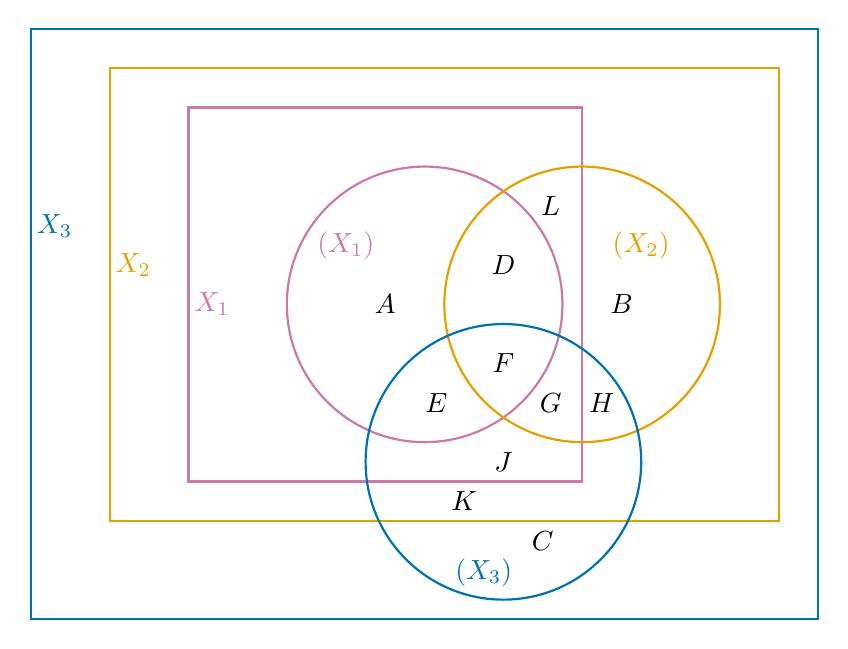
\begin{tikzpicture}
  \definecolor{colorone}{RGB}{204,121,167}
  \definecolor{colortwo}{RGB}{230,159,0}
  \definecolor{colorthree}{RGB}{0,114,178}

  \draw[colorthree, thick] (0,0.5) rectangle (10,8);
  \node[colorthree] at (0.3,5.5) {$X_3$};

  \draw[colortwo, thick] (1,1.75) rectangle (9.5,7.5);
  \node[colortwo] at (1.3,5) {$X_2$};

  \draw[colorone, thick] (2,2.25) rectangle (7,7);
  \node[colorone] at (2.3,4.5) {$X_1$};

  \draw[colorone, thick] (5,4.5) circle (1.75);
  \node[colorone] at (4,5.25) {$\choice(X_1)$};

  \draw[colortwo, thick] (7,4.5) circle (1.75);
  \node[colortwo] at (7.75,5.25) {$\choice(X_2)$};

  \draw[colorthree, thick] (6,2.5) circle (1.75);
  \node[colorthree] at (5.75, 1.1) {$\choice(X_3)$};

  \node at (4.5,4.5) {$A$};     %
  \node at (7.5,4.5) {$B$};     %
  \node at (6.5,1.5) {$C$};     %
  \node at (6,5) {$D$};     %
  \node at (5.15,3.25) {$E$};     %
  \node at (6,3.75) {$F$};     %
  \node at (6.6,3.25) {$G$};     %
  \node at (7.25,3.25) {$H$};       %
  \node at (6,2.5) {$J$};       %
  \node at (5.5,2) {$K$};     %
  \node at (6.6,5.75) {$L$};       %

\end{tikzpicture}
\caption{A set diagram with subsets labeled, for the proof of \Cref{thm:triangle-ineq}.}
\label{fig:choice-sets}
\end{figure}
Plugging these sets into the $r_\choice$ formula, we have

\begin{align*}
    r_\choice(X_1, X_3) & = |X_1 \cap \choice(X_3) \setminus \choice(X_1)| + |\choice(X_1) \setminus \choice(X_3)| & = |J \cup G| + |A \cup D|  \\
    r_\choice(X_1, X_2) & = |X_1 \cap \choice(X_2) \setminus \choice(X_1)| + |\choice(X_1) \setminus \choice(X_2)| & = |L \cup G| + |A \cup E|  \\
    r_\choice(X_2, X_3) & = |X_2 \cap \choice(X_3) \setminus \choice(X_2)| + |\choice(X_2) \setminus \choice(X_3)| & = |E \cup J \cup K| + |L \cup D \cup B| \\
\end{align*}

Recall that set union is such that %
for any finite sets $X, Y$, $|X| \leq |X \cup Y| \leq |X| + |Y|$.
Then it becomes clear that
\begin{align*}
    |J \cup G| + |A \cup D| & \leq |J| + |G| + |A| + |D| \\
    & \leq |E \cup J \cup K| + |L \cup G| + |A \cup E| + |L \cup D \cup B| \\
    r_\choice(X_1, X_3) & \leq r_\choice(X_1, X_2) + r_\choice(X_2, X_3)
\end{align*}
\end{proof}

\subsection{0-Instability}\label{sec:0-unstable-appendix}

\begin{restatable}[$0$-Instability]{definition}{zerostability}
\label{def:zero-instability}
Choice function $\choice$ is 0-unstable if and only if $r_\choice(X_1, X_2) = 0$ for all $X_1 \subseteq X_2$.
\end{restatable}

This describes realizable machine learning settings, where labels do not change as a result of shifts in the applicant pool.

\begin{restatable}{corollary}{Zero-Distance}
\label{thm:sub-mon-zero}
Choice function $\choice$ is 0-unstable if and only if it is both substitutable and monotonic.
\end{restatable}


This immediately follows from the two terms comprising $r_\choice$ mapping onto substitutability and monotonicity.

\subsubsection{Independence}

\begin{restatable}{definition}{Independence}
\label{def:independence}
$\choice$ is independent if for
 for all $x$,
either $x \in \choice(X)$
or $x \not\in \choice(X)$ for all $X$ where $x \in X$.
\end{restatable}

In other words, any element is either always accepted, or always rejected, when available, irrespective of the other elements available in a set $S$.

\subsubsection{Equivalence}

\begin{restatable}{theorem}{Independent Rules are Substitutable and Monotonic}
\label{thm:independent-sub-mon}
$\choice$ is independent if and only if it is both substitutable and monotonic.
\end{restatable}

\textit{Intuition}: The only way for adding applicants to neither hurt those already accepted or help those already rejected is to not affect them at all.
\begin{proof}
    Assume $\choice$ is independent.

    \textbf{Informal}
    Consider how independence implies substitutability and monotonicity. Independence means any element is always accepted or always rejected regardless of applicant pool. Then any $x$ that is accepted in $X_1$ is still accepted in any subset of $X_1$, which satisfies the definition of substitutability, and is accepted in any superset of $X_1$, which satisfies monotonicity.

    To prove that substitutability and monotonicity combine to form independence, consider the behavior they cover. Recall the intuition behind substitutability --- removing applicants does not lead to rejecting those accepted, and the intuition behind monotonicity --- adding applicants does not lead to rejecting those accepted. Given both properties, nothing can affect an acceptance decision at all.

    \textbf{Formal}
    First, we assume independence and prove $0$-stablility.
    Recall \Cref{lem:substitutability-term}: $\choice$ is substitutable if and only if $|X_1 \cap \choice(X_2) \setminus \choice(X_1)| = 0$ for all $X_1 \subseteq X_2$. Then for any $x \in X_1$, either $x \in \choice(X_1),\choice(X_2)$ or $x \not\in \choice(X_1),\choice(X_2)$, so $X_1 \cap \choice(X_2) = \choice(X_1)$. Then $|X_1 \cap \choice(X_2) \setminus \choice(X_1)| = 0$ and so $\choice$ is substitutable. Similarly, recall \Cref{lem:monotonicity-term}: $\choice$ is monotonic if and only if $|\choice(X_1) \setminus \choice(X_2)| = 0$ for all $X_1 \subseteq X_2$. Any element $x \in \choice(X_1)$ is in $X_2$ because $\choice(X_1) \subseteq X_1 \subseteq X_2$. By definition of independence, $x \in \choice(X)$ for all $X$ where $x \in X$, so if $x \in \choice(X_1)$, $x \in \choice(X_2)$, so $\choice(X_1) \subseteq \choice(X_2)$.

    To prove that substitutability and monotonicity together imply independence, consider any $x \in X$. If $x \in \choice(X)$, we can show that $x \in \choice(X')$ for any $X'$ where $x \in X'$. By monotonicity, $x \in \choice(X' \cup X)$, and so by substitutability, $x \in \choice(X')$. If $x \not\in \choice(X)$, we can prove $x \not\in \choice(X')$ for any $X'$. If we assumed for contradiction that $x \in \choice(X')$, then the same argument as above proves $x \in \choice(X)$, leading to contradiction.
\end{proof}

\begin{restatable}{corollary}{Only Independent Rules are 0-unstable}
\label{thm:independent-zero-unstable}
$\choice$ is $0$-unstable if and only if it is independent, and therefore no $q$-acceptant $\choice$ can be $0$-unstable.
\end{restatable}

This immediately follows from $\Cref{thm:sub-mon-zero}$, $\Cref{thm:independent-sub-mon}$, and $\Cref{thm:mono-accept-mutex}$.

\subsection{1-Instability} \label{sec:1-unstable-appendix}

\subsubsection{Equivalence with Substitutability} \label{sec:sub-equiv-proof}

\begin{restatable}[Substitutability and 1-Instability are Equivalent Under Capacity Constraints]{theorem}{subequiv}
\label{thm:sub-unstable-equiv}
Any $q$-acceptant choice function is $1$-unstable if and only if it is substitutable.
\end{restatable}

\begin{proof}
\textbf{Informal}
Intuitively, $q$-acceptance means that every acceptance decision that becomes a rejection must also be paired with a new acceptance to keep the size of the accepted set the same. Substitutability implies that adding elements cannot cause new acceptances from rejections, so the only possible newly accepted element is the newly added one.

Recall that the first term of $r_\choice$ is always zero only for substitutable $\choice$. So, we only need to show $|\choice(X) \setminus \choice(X')| \leq 1$ if and only if $\choice$ is substitutable. %
First, we show that $\choice$ being substitutable is \textit{sufficient} for $1$-instability. If $\choice$ is substitutable, then all elements in $\choice(X')$ except for $x'$ must be in $\choice(X)$. By $q$-acceptance, $|\choice(X')| = |\choice(X)| = q$ (the $|X| < q$ case is trivial), so $\choice(X)$ can have at most one element not in $\choice(X')$, making $\choice$ 1-unstable.

Second, we show that substitutability is \textit{necessary} for $1$-instability. If $\choice$ is not substitutable, there is some $X \subseteq X'$ and $x^* \in X$ such that $x^* \notin \choice(X)$ but $x^* \in \choice(X')$ (by \Cref{lem:unsubstitutable}). This creates one change. By $q$-acceptance, this forces another candidate out of $\choice(X')$, creating at least a second change, violating 1-instability.

Together, these show that under $q$-acceptance, substitutability is necessary and sufficient for $1$-instability, completing the proof.
\end{proof}


\begin{restatable}{theorem}{BoundedDistance}
\label{thm:sub-accept-consistent}
Any $q$-acceptant, substitutable $\choice$ is consistent.
\end{restatable}

\begin{proof}
Consider $X_1, X_2$ where $\choice(X_2) \subseteq X_1 \subseteq X_2$ for substitutable, $q-$acceptant $\choice$. Substitutability guarantees that if $x \in \choice(X_2)$ and $x \in X_1$, $x \in \choice(X_1)$. By construction, this applies to all $x \in \choice(X_2)$, because $\choice(X_2) \subseteq X_1$; therefore, $\choice(X_2) \subseteq \choice(X_1)$. As $|\choice(X_2)| = |\choice(X_1)|$, and $\choice(X_1),\choice(X_2)$ are finite sets, this means that $\choice(X_2) = \choice(X_1)$, which is the definition of consistency.
\end{proof}

\subsection{\textit{d}-Instability} \label{sec:d-unstable-appendix}

\subsubsection{Proof of \Cref{lem:unstable-calc}} \label{sec:calc-proof}

\begin{restatable}[Calculating Instability]{lemma}{stablecalc}
\label{lem:unstable-calc}
For all $q$-acceptant $\choice$, let $X' = X \cup \{x'\}$ for $|X| \geq q$ and $n = |\choice(X) \setminus \choice(X')|$.  Then
$r_\choice(X, X') = 2n-\mathbf{1}_{x'\in\choice(X')}$.
\end{restatable}

\begin{proof}
\textbf{Informal}
If input sets differ by one element, but the selected sets differ by $n$ elements, then it must be that $n$ previously accepted elements were rejected and there must be $n$ new accepted elements, at least $n-1$ must have been previously rejected, because the size of the accepted set is fixed.

\textbf{Formal}
By $q$-acceptance, $|\choice(X)| = |\choice(X')| = q$. Then $|\choice(X) \setminus \choice(X')| = |\choice(X') \setminus \choice(X)| = q-|\choice(X) \cap \choice(X')|$.
Second, note that $\choice(X') \setminus \choice(X) = (\choice(X') \cap X) \setminus \choice(X)$ if $x' \not\in \choice(X')$, and otherwise $\choice(X') \setminus \choice(X) = \{x'\} \cup \left((\choice(X') \cap X) \setminus \choice(X)\right)$.
Putting the previous statements together, we get two cases:
\begin{itemize}
    \item $x' \not\in \choice(X')$: $|\choice(X) \setminus \choice(X')| = |\choice(X') \setminus \choice(X)| = |X \cap \choice(X') \setminus \choice(X)|$
    \item $x' \in \choice(X')$: $|\choice(X) \setminus \choice(X')| = |\choice(X') \setminus \choice(X)| = |X \cap \choice(X') \setminus \choice(X)| + 1$
\end{itemize}
Then $r_\choice(X, X') = |X \cap \choice(X') \setminus \choice(X)| + |\choice(X) \setminus \choice(X')| = 2|X \cap \choice(X') \setminus \choice(X)| + \mathbf{1}_{x'\in\choice(X')} = 2|\choice(X) \setminus \choice(X')| - \mathbf{1}_{x'\in\choice(X')}$
\end{proof}

\begin{example}
Suppose applicants are each one of at least
$n$ different types (e.g. instrument specializations) and suppose they also have an overall ``talent'' rating.
Then suppose that admissions is determined by forming complementary groups of size $n$ (e.g. quartets) to the extent possible, and is otherwise based on a single ``talent'' rating.
Suppose type 1 candidates are the bottleneck in forming groups.
Then one additional type 1 candidate in the applicant pool allows one additional group to be admitted ($n$ new admits). By \Cref{lem:unstable-calc}, this rule cannot be $d$ unstable for $d<2n-1$.
\end{example}

\subsubsection{Inconsistent Instability}\label{sec:inconsistent-proof}

\begin{restatable}[Even Instability is Inconsistent]{theorem}{inconsistentstable}
\label{thm:even-inconsistency}
For any $q$-acceptant $\choice$, $\choice$ is inconsistent if and only if there exist $X, X' = X \cup \{x'\}$ where $r_\choice(X, X')$ is positive and even.
\end{restatable}

\textit{Intuition}: for $\choice$ to have an even but nonzero choice distance $r_\choice$, the indicator term in  \Cref{lem:unstable-calc} must be zero; the added $x'$ is not selected. But that means $x'$ is a rejected element that still has an impact, which violates consistency.
\begin{proof}
\textbf{Informal}
First, we prove that an even and positive value of $r_\choice$ implies inconsistency. For $\choice$ to have an even but nonzero choice distance $r_\choice$, the indicator term in  \Cref{lem:unstable-calc} must be zero; the added $x'$ is not selected. But that means $x'$ affects selection without actually being chosen, which violates consistency.

Next, prove that consistency limits the values of $r_\choice$. If $\choice$ is not consistent, then there is some $X, X'$ where the new element $x'$ is not chosen (so the indicator term in \Cref{lem:unstable-calc} is zero and $r_\choice$ is even), but changes the chosen elements. This makes  $r_\choice$ is positive under a fixed capacity constraint.

\textbf{Formal}
Consider \Cref{lem:unstable-calc}. See that for $r_\choice \neq 0$, $r_\choice$ is odd if and only if $x' \in \choice(X')$ and even if and only if $x' \not\in \choice(X')$. If $x' \not\in \choice(X')$, then $\choice(X') \subseteq X$. %
So if $x' \not\in \choice(X')$ but $n > 0$, $\choice(X') \subseteq X$ but $\choice(X') \neq \choice(X)$, which proves inconsistency.
Similarly, if $\choice$ is inconsistent, there is $\choice(X') \subseteq X$ but $\choice(X') \neq \choice(X)$. %
As $\choice(X') \neq \choice(X)$, $n > 0$, but for $\choice(X') \subseteq X$ to be true, $x' \neq \choice(X')$, and so $r_\choice(X, X')$ is even.
\end{proof}

\begin{restatable}{corollary}{No Consistent Tightly Even Instability}
\label{cor:even-inconsistency}
There is no $q$-acceptant and consistent $\choice$ that is tightly $dk$-unstable for even values of $d$.
\end{restatable}

This follows directly from \Cref{thm:even-inconsistency}.

While inconsistent choice functions are generally less intuitive (and formally studied much less), there exist some real-world examples of inconsistent choice functions. Famously, voting theory is rife with spoiler effects, where adding a dummy candidate changes the selected outcome. Consider the choice function in the US presidential election of 1912. Say that with the candidate pool being just William Taft and Woodrow Wilson, Taft would win (Wilson only got 41\% of votes). However, adding Theodore Roosevelt to the ballot led to Wilson winning, which violates consistency.
More relevantly to our setting, some schools value student uniqueness. We could imagine cases where a university admits a student because their niche interest is particularly noteworthy, but if multiple have this interest, they may end up taking none. Similarly, if only one student from an unknown high school applies to a university, they may stand out more than if every student from that school applied.

\subsection{Proof of \Cref{thm:instability}} \label{sec:instability-proof}

Recall \Cref{thm:instability}:
\thminstability*

Putting things together, the first statement of \Cref{thm:instability} comes from \Cref{thm:independent-zero-unstable} and the second from \Cref{thm:sub-unstable-equiv}. The third
has roots in \Cref{lem:unstable-calc}, which allows us to calculate instability.

Rigorously, we can generate a $d$-unstable $\choice$ for any $1 < d \leq 2q$. Take any $1$-unstable, $q$-acceptant $\choice$ induced by a total order $\succ$ (i.e, is a ranking). Let $n$ be $\frac{d}{2}$, rounded down. Then let $X^* = \{x^*_1, ..., x^*_n\}$ be the $n$ \textit{minimal} elements of $\succ$ (or any $n$ elements that are not among the $n$ maximal elements, if there exist any.) Then modify $\choice$ such that if $X^* \subseteq X$ for any input $X$, $X^* \subseteq \choice(X)$. Then $\choice$ is tightly $2n-1$-unstable. To make $\choice$ $2n$-unstable, let there be some $x'$ such that if $X^* \subseteq X$ but $x' \in X$ as well, then \textit{no} element of $X^*$ is in $\choice(X)$. %

The intuition for the construction is that $X^*$ forms a highly desirable team, even though each element is not individually desirable, nor are partial subsets of $X^*$.
In the inconsistent case (even instability) $x'$ represents a candidate whose mere presence negates the value of $X^*$ as a team, even when not accepted.

\subsection{Variability} \label{sec:variability-appendix}

\subsubsection{Generalizing and Justifying Variability}

In \Cref{sec:theory-definitions}, we provide a definition of variability for $1$-unstable, $q$-acceptant functions. Here, we provide a more thorough justification of \Cref{def:variability} by reducing it from a more general and nuanced characterization.
Notably, instability counts how many admissions decisions change when an applicant is added \textbf{or} removed. The definition in \Cref{def:variability}, however, focuses only on the case of \textbf{adding} elements. In the general case, there are two relevant sets, defined when adding or removing an element.

As per \Cref{def:variability}, when appending a new element to the input set $X$, different applicants may become rejected: let the set of ``borderline admits'' $V_\choice(X)$ be
\begin{equation}
V_\choice(X) = \bigcup\limits_{x'\in\calX} \choice(X) \setminus \choice(X \cup \{x'\})
\end{equation}
which we shall call the ``borderline set'' for short. Notice that this is bounded by $q$, as $|\choice(X)| = q$.

Conversely, when removing an applicant from $X$, let the set of applicants that might be newly accepted be
\begin{equation}
A_\choice(X) = \bigcup_{x^*\in X} \choice(X \setminus \{x^*\}) \setminus \choice(X)
\end{equation}
the set of ``waitlisted rejections''; likewise, we shall call this the ``waitlisted set''.

\begin{definition}[Variability, General]
\label{def:variability-general}
A choice function $\choice$ has \textit{variability} $m$ where:
$$m := \max\left\{\max_{X\subset \calX} \left|V_\choice(X)\right|, \max_{X\subset \calX} \left|A_\choice(X)\right| \right\}$$
\end{definition}

\textit{Intuition}: Variability bounds how many different currently accepted candidates could potentially be displaced by adding any single new candidate \textit{or} how many different candidates are newly accepted if a currently accepted candidate is removed.%

\subsubsection{Equivalence in the 1-unstable Case} \label{sec:var-proof}

Here, we show that, for capacity-constrained, substitutable functions in large universes, the general definition in \Cref{def:variability-general} reduces to \Cref{def:variability}.

\begin{restatable}{theorem}{appendremove}
\label{thm:append-remove-size}
For $q$-acceptant, 1-unstable $\choice$, and $|\calX| \geq 2q$, the maximum size of the waitlisted set is equal to the maximum size of the borderline set; that is,
\begin{equation}
\max_{X\subset \calX} \left| V_\choice(X)\right| = \max_{X\subset \calX} \left| A_\choice(X)\right|
\end{equation}
\end{restatable}

In short, if there is a set $X$ with a waitlisted set of size $u$, there must be a set $X_0$ with a borderline set of size (at least) $u$, and vice versa. %

\begin{proof}
To prove equality, we will prove that 1) $\max_{X\subset \calX} \left| V_\choice(X)\right| \geq \max_{X\subset \calX} \left| A_\choice(X)\right|$ and then that 2) $\max_{X\subset \calX} \left| V_\choice(X)\right| \leq  \max_{X\subset \calX} \left| A_\choice(X)\right|$.

\textbf{Part 1).}
To prove the first statement, assume that there is some $X$ where the waitlisted set is of cardinality at least $u$, so $x^*_1, ..., x^*_u \in A_\choice(X)$.

Then (recall that $\choice$ is consistent) there are $X_1, ..., X_u \subseteq X$ where $X_i = X \setminus \{x'_i\}$ such that $\choice(X_i) = x^*_i \cup \choice(X) \setminus x'_i$ for $i \in \{1, ..., u\}$. Then consider $X_0 = \bigcap_{i=1}^u X_i = X \setminus \{x'_1, ..., x'_u\}$, and $\choice(X_0)$. It must be that $\choice(X_0) = \{x^*_1, ..., x^*_u\} \cup \choice(X) \setminus \{x'_1, ..., x'_u\}$ by substitutability. I claim that $\{x^*_1, ..., x^*_u\} \subseteq V_\choice(X_0)$, which means $|V_c(X_0)| \geq u$, which would complete the proof.

Assume for contradiction that this is untrue; $\{x^*_1, ..., x^*_u\} \not\subseteq V_\choice(X_0)$. Then some $x^*_i$, say $x^*_u$ (without loss of generality), is not in $V_\choice(X_0)$, which means that $x^*_u \in \choice(\{x'_u\} \cup X_0)$.
Consider the makeup of $\choice(\{x'_u\} \cup X_0)$. Recall that $\{x'_u\} \cup X_0 = \bigcap_{i=1}^{u-1} X_i = X \setminus \{x'_1, ..., x'_{u-1}\}$. Because of substitutability, as a subset of $X$, we have $\left(\choice(X) \setminus \{x'_1, ..., x'_{u-1}\}\right) \subseteq \{x'_u\} \cup X_0$. From substitutability, as a subset of from $X_1$ through $X_{u-1}$, $\{x^*_2, ..., x^*_{u-1}\}$ are likewise chosen.
However, consider the size of $\choice(\{x'_u\} \cup X_0)$. $|\choice(X) \setminus \{x'_1, ..., x'_{u-1}\}|$ is of size $q-(u-1)$, because $x'_i \in \choice(X)$ for all $i$. We also know that $|\{x^*_1, ..., x^*_{u-1}\}| = u-1$, and as no  $x^*_i$ is in $\choice(X)$ by definition, all of these elements are distinct. As $x^*_u$ remains by assumption, this adds up to $|\choice(\{x'_u\} \cup X_0)| = q+1$, which violates $q$-acceptance and completes the proof.

\textbf{Part 2).}
The proof for 2) is extremely similar to the former. Begin with $X_0$ with $V_\choice(X_0) = \{x^*_1, ..., x^*_m\}$, with $x'_1, ..., x'_m$ such that $\choice(X'_1) = \{x'_1\} \cup \choice(X_0) \setminus \{x^*_1\}$. Let $X = \bigcup_{i=1}^m /X'_i = X_0 \cup \{x'_1,...,x'_m\}$ and $X_i = X \setminus \{x'_i\}$. Note that $X_i = X'_1 \cup ... X'_{i-1} \cup X'_{i+1} \cup ... \cup X_m$. %
Because of $1$-instability, $|\choice(X_0) \setminus \choice(X)| \leq |X_0 \setminus X| = m$. Because of substitutability, any $x \in \choice(X)$ is either in $\choice(X_0)$ or not in $X_0$ and therefore in $\{x'_1, ..., x'_m\}$.

I claim $\choice(X) = \{x'_1,...,x'_m\} \cup \choice(X_0) \setminus \{x^*_1,..., x^*_m\}$. Firstly, $x^*_i \not\in \choice(X)$ because  $x^*_i \not\in \choice(X'_i)$ and $X'_i \subseteq X$, so that would be a substitutability violation. As $\choice(X_0) \setminus \{x^*_1,..., x^*_m\}$ has $q-m$ elements, the only possible elements to fill $\choice(X)$ must be the $m$ elements of $\{x'_1,...,x'_m\}$.

The same argument holds for any $X_i$, but use $X_m$ without loss of generality for ease of notation; $X'_j \subseteq X_m$ for $m \neq j$, so $x^*_j \not\in\choice(X_m)$ by substitutability. With $\choice(X_0) \setminus \{x^*_1,..., x^*_{m-1}\}$ being the only $q-m+1$ elements of $X_0$ that can be in $\choice(X_m)$, the other $m-1$ elements must be $\{x'_1,. .., x'_{m-1}\}$. Then consider the definition of $A_\choice(X)$ and see that $\choice(X \setminus x'_i) \setminus \choice(X) = \{x^*_i\}$ for any $i$, with each $x^*_i$ being unique.
\end{proof}

\subsection{Queues and 1-Variability}\label{sec:ranking-proof}

\subsubsection{Some Lemmas}

\begin{restatable}[Consistency of Removable Sets]{lemma}{consistentremove}
\label{lem:consistent-remove}
Let $\choice$ be 1-unstable and q-acceptant with variability $m$. For any $X_1, X_2$, if $\choice(X_1) = \choice(X_2)$, then $V_\choice(X_1) = V_\choice(X_1)$.
\end{restatable}

\begin{proof}
Recall from \Cref{thm:sub-accept-consistent} that $\choice$ must be consistent and so $\choice(\choice(X)) = \choice(X)$ for any $X$.

Consider any $x'$ associated with an element $x^*$ of $V_\choice(X)$, such that $\choice(X) \setminus \choice(X') = \{x^*\}$ (and even more precisely, by $q$-acceptant substitutability, that $\choice(X') = \{x'\} \cup \choice(X) \setminus \{x^*\}$ exactly). Note that $\choice(X') \subseteq \choice(X) \cup \{x'\} \subseteq X'$, and therefore $\choice(\choice(X) \cup \{x'\}) = \choice(X')$ by consistency. This applies to all possible $x'$ (including when $x' \in X$), and therefore, $V_\choice(X) = V_\choice(\choice(X))$.

As this set equality is exact, apply this logic to some $X_2$ and see $V_\choice(X_1) = V_\choice(\choice(X_1)) = V_\choice(\choice(X_2)) = V_\choice(X_2)$.
\end{proof}

\begin{restatable}{lemma}{Ranking m}
\label{lem:a-v-equal}
Let $q$-acceptant, $1$-unstable $\choice$ have variability $1$. Then $V_\choice(X) = A_\choice(X \cup \{x'\})$ when $\choice(X \cup \{x'\}) \neq \choice(X)$.
\end{restatable}

\begin{proof}
If $\choice(X \cup \{x'\}) \neq \choice(X)$, then $\choice(X \cup \{x'\}) = \{x'\} \cup \choice(X) \setminus x^*$ where $V_\choice(X) = \{x^*\}$ (by consistency, 1-instability, and the definition of variability). Then $X' \setminus \{x'\}) = X$ and so $A_\choice(X') = \{x^*\}$, completing the proof.
\end{proof}

\subsubsection{Equivalence of Queues and $1$-variability}
Here we present the proof for $1$-unstable $1$-variability being equivalent to $q$-representativeness, i.e., being fully characterized by a total order.

\begin{restatable}[$q$-Representativeness and $1$-Variability are Equivalent]{theorem}{rankingvariability}
\label{thm:ranking-variability}
$\choice$ is $q$-representative if and only if it is $q$-acceptant and $1$-unstable with variability $1$.
\end{restatable}
\begin{proof}
We prove this in two parts: first, that $q$-representativeness implies $1$-variability, and then the converse.

\paragraph{Direction 1} %
Note that $q$-representativeness implies $q$-acceptance by definition.

Next, we prove that $q$-representativeness implies $1$-instability. Assume for contradiction that some $q$-representative $\choice$ is not substitutable (and therefore not $1$-unstable). Then there exists (by \Cref{lem:unsubstitutable}) some $x^*$, $x'$, $X$ and $X' = X \cup \{x'\}$ where $x^* \in X$ and $x^* \in \choice(X')$ but $x^* \not\in \choice(X)$. By $q$-acceptance, there must be at least one $x$ in $\choice(X)$ that is not in $\choice(X')$ (which must take the place of $x^*$). However, $\choice(X')$ implies that $x^* \succ x$, while $\choice(X)$ implies that $x \succ x^*$ --- violating asymmetry and leading us to contradiction.

Lastly, proving that $q$-representative $\choice$ leads to $m=1$ is relatively intuitive. For any $X$, $\choice(X)$ are the $q$ highest-ranked elements of $X$. Denote $X = \{x_1, x_2, ..., x_k\}$ where $|X| = k$ and $x_1 \succ x_2 \succ ...\succ x_k$. Then $\choice(X) = \{x_1, ..., x_{q^*}\}$ where $q^* = \min\{q, k\}$.
Assume for contradiction that there is a $q$-representative $\choice$ with variability $m > 1$. Then there exists some $X$ where $|V_\choice(X)| > 1$; say that $\{x^*_a, x^*_b\} \subseteq V_\choice(X)$. Then there exists some $x'_a$ where $\choice(X) \setminus \choice(X \cup x'_a) = \{x^*_a\}$ and similar $x'_b$ for $x^*_b$. The first implies $x^*_b$ is ranked above $x^*_a$, but the second implies the opposite. Then choices cannot be made according to a static ranking and $\choice$ is not $q$-representative, completing the proof by contradiction. %

\paragraph{Direction 2}
Assume $q$-acceptance, variability 1, and instability 1. Now we prove $\choice$ is $q$-representative. To be precise, I take this to mean that $\choice$ is indistinguishable from some $q$-representative $\choice$; $\choice$ could be represented by some total ordering over elements of $X$. We show this strict total ordering constructively.

Define $\succ$ such that, if $x_a \in \choice(X)$ but $x_b \not\in\choice(X)$ for any $x_a, x_b \in X$, $x_a \succ x_b$. Note that this implies that the existence of some set $A$ where $x_a \in \choice(A)$ and $A_\choice(A) = \{x_b\}$ by consistency (e.g. $A = \choice(X) \cup \{x_b\}$). This also implies $A'$ where $x_a, x_b \in \choice(A')$, $V_\choice(A') = \{x_b\}$, where $A' = A \setminus \{x\}$ for any $x \neq x_a, x_b$.

Then, we need to prove this relation is asymmetric, transitive, and completeness (or rather, is indistinguishable from a complete relation when examining the induced choice function).

\paragraph{Asymmetry}
First, we show asymmetry. Assume for contradiction that $a \succ b$ and $b \succ a$. Then there exists $X_a$ where $a, b \in X_a$, $a \in \choice(X_a)$ and $b \not\in \choice(X_a)$, and a similar $X_b$ where $a \not\in \choice(X_b)$ and so on.

Let $X_a = \choice(X_a) \cup \{b\}$ (we can construct such out of any $X_a$, by consistency), where $A_\choice(X_a) = \{b\}$, and denote $\choice(X_a) = \{x^a_1, ..., x^a_{q-1}, a\}$. Construct $X_b$ similarly. Further, let $X'_a = X_a \setminus \{x^a_1\}$, and note that $V_\choice(X_a') = \{b\}$.

Then from here, we add the elements of $X_b$ to $X_a'$, constructing $X_1, X_2,$ and so forth.

Let $X_0 = X_a'$ and sequentially construct a series of $X_t$. Add $x^b_t$ to $X_{t-1}$. If $x_b \not\in \choice(X_{t-1} \cup \{x^b_t\})$, then let $X_t = X_{t-1} \cup \{x^b_t\}$, and $V_\choice(X_t) = \{b\}$ by \Cref{lem:consistent-remove}. If $x^b_t \in \choice(X_{t-1} \cup \{x^b_t\})$, then $b \not\in \choice(X_{t-1} \cup \{x^b_t\})$ and $A_\choice(X_{t-1} \cup \{x^b_t\}) = \{b\}$ (by \Cref{lem:a-v-equal}). Then let $X_t = \{x^b_t\} \cup X_a' \setminus x^a_i$ where $x^a_{i-1} \not\in X_{t-1}$ but $x^a_i \in X_{t-1}$, and $V_\choice(X_t) = \{b\}$ (again, by \Cref{lem:a-v-equal}). Note that $a \in \choice(X_t)$, $b \in X_t$, and specifically $b \in V_\choice(X_t)$, for all $t \in \{0,..., q-2\}$.

Then $X_{q-2}$ will contain $x^b_1,...x^b_{q-2}$. Let $X^* = X_{q-2} \cup \{x^b_{q-1}\}$. Note that adding $x^b_{q-1}$ to $X_{q-2}$ makes $X^* \supseteq X_b$. Then, if $a \in \choice(X^*)$, substitutability is violated, as $a \not\in \choice(X_b)$. If $x^b_{q-1} \not\in \choice(X^*)$, then $\choice(X_{q-2}) = \choice(X^*)$ by consistency, and $a \in \choice(X_{q-2})$. If instead $x^b_{q-1} \in \choice(X^*)$, recall that $V_\choice(X_{q-2}) = \{b\}$, so $a \not\in V_\choice(X_{q-2})$, and $a$ remains in $\choice(X^*)$. Therefore, either possibility leads to contradiction, proving that $\succ$ is asymmetric.

\paragraph{Transitivity}
Say that $a \succ b$ and $b \succ c$ and we want to prove $a \succ c$. If $a \succ b$, there exists some $X$ where $a, b \in X$, $a \in \choice(X)$, and $b \not\in \choice(X)$. Let $X$ be $\choice(X) \cup \{b\}$, where $a \in \choice(X), b \not\in\choice(X)$ by consistency. Then consider $X \cup \{c\}$. By asymmetry, $c \not\succ b$, so $c \not\in \choice(X\cup \{c\})$. By consistency, then, $\choice(X\cup \{c\}) = \choice(X)$, so $a \in \choice(X\cup \{c\})$ and $a \succ c$, completing the proof.

\paragraph{(Almost)-Completeness}
See that this relation must exist for all but $q$ elements --- and any arbitrary linear extension thereof generates the same choice function behavior.

For any $a, b$, let there be some $X_0$ where $a, b \not\in \choice(X_0)$. Then remove elements of $\choice(X_t)$ in a sequence $X_0, ..., X_t$ until $A_\choice(X_t) = \{a\}$ or $\{b\}$. This must happen for some value of $t$ because when $|X_t| = q+1$, at least one of $a$ or $b$ are in $\choice(X)$, and due to $1$-instability, both $a$ and $b$ cannot be added to $\choice(X_t)$ at once. The only exception is if there is no such $X_0$ where $a, b \not\in \choice(X_0)$, which can only be true if $a$ is such that $a \in \choice(X)$ for all $X$ (and similarly for $b$). (If $a \not\in \choice(X)$ for some $X$, then substitutability implies $a \not\in \choice(X \cup \{b\})$). However, there can only be $q$ such elements (by $q$-acceptance). Note that any linear extension of this partial order will produce the same choice function behavior; that is, any constructed total ordering that otherwise aligns with $\succ$ will produce the same choice behavior, and thus, $\choice$ can be represented by any such strict total ordering.
\end{proof}

\subsection{Higher-Variability Functions} \label{sec:high-variability-appendix}
In this subsection, we examine two different cases of choice functions: those that are sequentially composed of other choice functions, and those that can be represented as a linear assignment problem (also described in graph-theoretic terms as a maximum- or minimum-weight bipartite matching).

\subsubsection{Sequential Composition} \label{sec:seq-proofs}
A useful class of choice functions are choice functions that can be broken down or defined as a sequential composition of functions $\choice_n, \choice_{n-1}, ..., \choice_1$; that is,
$\choice(X) = \choice_n(X) \cup \choice_{n-1}(X_{n-1}) \cup ... \cup \choice_1(X_1)$ where $X_i = X_{i+1} \setminus\choice_{i+1}(X_{i+1})$ and $X_n = X$. Sequential composition is particularly useful because it preserves a variety of useful properties. Sequences of $q_i$-acceptant functions are $q$-acceptant, because no duplicate elements are selected by multiple functions, and therefore preserves $q$-acceptance when each function in the sequence has capacity $q_i$ (i.e., $q = q_n + ... + q_1$.)
\seqcomposition*

\textit{Intuition}: Selection proceeds in stages, with each stage operating on candidates not selected by higher-priority stages.

\paragraph{Sequentially Composed Substitutable Functions Are Substitutable}
Similarly, we show sequential compositions of substitutable functions are also substitutable.
\begin{restatable}[Composition Preserves Substitutability]{theorem}{seqsub}
\label{thm:composition-substitutable}
Sequential composition of substitutable functions yields a substitutable function.
\end{restatable}

\textit{Intuition}:
``Appending'' a substitutable choice function $\choice_2$ before another substitutable function $\choice_1$ affects the inputs to $\choice_1$ in a structured way.
\begin{proof}
    Proof by induction.
    In the base case, for $n = 1$, $\choice(X) = \choice_1(X)$, and as $\choice_1$ is given to be substitutable, $\choice$ is as well.

    For the inductive step, show that $\choice^{n+1}$ is substitutable when comprised of $\choice_{n+1}, \choice_n, ..., \choice_1$, assuming that $\choice^n$ comprised of $\choice_n,...,\choice_1$ is substitutable.

    The definition of substitutability is that $X \subseteq X'$ implies $\choice(X') \cap X \subseteq \choice(X)$. So we need to show $\choice^{n+1}(X') \cap X \subseteq \choice^{n+1}(X)$.

    First, note that $\choice^{n+1}(X) = \choice_{n+1}(X) \cup \choice^n(X \setminus \choice_{n+1}(X))$.
    Let $S = X \setminus \choice_{n+1}(X)$ and $S' = X' \setminus \choice_{n+1}(X')$. As $S \subseteq X'$, we only need to show that no elements of $S$ are elements of $\choice_{n+1}(X')$. As $\choice_{n+1}$ is substitutable, $\choice_{n+1}(X') \cap X = \choice_{n+1}(X)$. So, any element of $X$ that is in $\choice_{n+1}(X') $ must be in $\choice_{n+1}(X)$, and therefore cannot be in $S = X \setminus \choice_{n+1}(X)$. Therefore, $S \subseteq S'$.

    Now, we can apply the induction hypothesis, so we assume $\choice^n$ is substitutable to get

    \begin{align*}
        \choice^n(S') \cap S & \subseteq \choice^n(S) && \text{induction hypothesis} \\
        \choice^n(S') \cap \left(X \setminus \choice_{n+1}(X)\right) & \subseteq \choice^n(S) &&  \text{substitute out $S$}\\      \left(\choice^n(S') \cap X\right) \setminus \left(\choice^n(S') \cap  \choice_{n+1}(X)\right) & \subseteq \choice^n(S) && \text{intersection commutes}\\
        \choice_{n+1}(X) \cup \left[\left(\choice^n(S') \cap X\right) \setminus \left(\choice^n(S') \cap  \choice_{n+1}(X)\right)\right] & \subseteq \choice_{n+1}(X) \cup \choice^n(S) && \text{add $\choice_{n+1}(X)$} \\ \intertext{Note that $\choice_{n+1}(X) \supseteq\left(\choice^n(S') \cap  \choice_{n+1}(X)\right)$, so the set difference can be simplified out:}
        \choice_{n+1}(X) \cup \left(\choice^n(S') \cap X\right) & \subseteq \choice_{n+1}(X) \cup \choice^n(S) && \text{equivalent} \\ \intertext{Note that for any sets $A,B,C$, $(A \cup B) \cap C = (A \cap C)\cup (B \cap C) \subseteq A \cup (B \cap C)$, so:
        }
        \left(\choice_{n+1}(X) \cup \choice^n(S') \right) \cap X & \subseteq \choice_{n+1}(X) \cup \choice^n(S) && \text{} \\
        \left(\choice_{n+1}(X) \cup \choice^n(X' \setminus \choice_{n+1}(X')) \right) \cap X & \subseteq \choice_{n+1}(X) \cup \choice^n(X \setminus \choice_{n+1}(X)) &&  \text{substitute out $S$, $S'$}  \\
        \choice^{n+1}(X') \cap X & \subseteq \choice^{n+1}(X) &&  \text{definition of $\choice^{n+1}$}
    \end{align*}

    Which is the definition of substitutability, completing the proof.
\end{proof}

\begin{restatable}[Additive Variability Bound]{theorem}{addvar}
\label{thm:additive-variability}
If $\choice$ is a sequential composition of $q$-acceptant, $1$-unstable functions with variabilities $m_1, \ldots, m_n$, then $\choice$ has variability at most $\sum_{i=1}^n m_i$.
\end{restatable}

Note that this is only an upper bound; we could trivially construct cases where this is not tight. For example, compose a $\choice$ of two $q$-representative choice functions with the same underlying ordering. On the other hand, it is also easy to construct instances in which this upper bound is tight. Consider the composition of $m$ queues which each rank a student by a different subject area exam. Then the addition of a new student to the applicant pool could displace any of $m$ students, depending on the subject area.

\textit{Intuition}:
The intuition of this proof lies in the fact that ``appending'' a 1-unstable function $\choice_2$ can ``contribute'' $m_2$ variability, and that perturbing the inputs to $\choice$ can only perturb the inputs to $\choice_1$ by the same amount because $\choice_2$ is $1$-unstable.
\begin{proof}
Proof by induction.

In the base case, for $n = 1$, $\choice(X) = \choice_1(X)$, so $m = m_1$.

For the inductive step, show that $\choice^{n+1}$ has variability $m' \leq m + m_{n+1}$ when comprised of $\choice_{n+1}, \choice_n, ..., \choice_1$, assuming that $\choice^n$ comprised of $\choice_n,...,\choice_1$ has variability $m$ and $\choice_{n+1}$ has variability $m_{n+1}$.

First, note that $\choice^{n+1}(X) = \choice_{n+1}(X) \cup \choice^n(X \setminus \choice_{n+1}(X))$.
Recall the definition of variability:
\[
m \coloneqq \max_{X\subset \calX} \left|\bigcup\limits_{x'\in\calX} \choice(X) \setminus \choice(X \cup \{x'\})\right|
\]

We are interested in $\bigcup\limits_{x'\in\calX} \choice^{n+1}(X) \setminus \choice^{n+1}(X \cup \{x'\})$ for every $X$.
For ease of notation, let $X' = X \cup \{x'\}$, $S = X \setminus \choice_{n+1}(X)$, and $S' = X' \setminus \choice_{n+1}(X')$.

\begin{align*}
    \bigcup\limits_{x'\in\calX} \choice^{n+1}(X) \setminus \choice^{n+1}(X')
    = & \bigcup\limits_{x'\in\calX} \left[\choice_{n+1}(X) \cup \choice^n(S)\right] \setminus \left[\choice_{n+1}(X') \cup \choice^n(S')\right] & \text{notation substitution}\\
    = & \bigcup\limits_{x'\in\calX} \left[\choice_{n+1}(X)  \setminus \choice_{n+1}(X')  \setminus \choice^n(S')\right] \cup \left[\choice^n(S) \setminus \choice_{n+1}(X')  \setminus \choice^n(S')\right]
    & \text{set diff distributes} \\
    = & \bigcup\limits_{x'\in\calX}  \left[\choice_{n+1}(X)  \setminus \choice_{n+1}(X')  \setminus \choice^n(S')\right] \cup \bigcup\limits_{x'\in\calX} \left[\choice^n(S) \setminus \choice_{n+1}(X')  \setminus \choice^n(S')\right] \\
    \subseteq & \bigcup\limits_{x'\in\calX}  \left[\choice_{n+1}(X)  \setminus \choice_{n+1}(X') \right] \cup \bigcup\limits_{x'\in\calX} \choice^n(S)\setminus \choice^n(S') \\
\end{align*}

So we have
\begin{equation*}
    \left|\bigcup\limits_{x'\in\calX} \choice^{n+1}(X) \setminus \choice^{n+1}(X \cup \{x'\}) \right| \leq \left|\bigcup\limits_{x'\in\calX}  \choice_{n+1}(X) \setminus \choice_{n+1}(X') \right| + \left| \bigcup\limits_{x'\in\calX} \choice^n(S)\setminus \choice^n(S')\right|
\end{equation*}

See that the left term is bounded precisely by the variability of $\choice_{n+1}$.
Next, we need to show that the right term is bounded by $m$.
To apply the variability bound to the right term, we need to show that $S' = S \cup \{x''\}$ for some $x''$ for all $S, S'$, which holds if $|S' \setminus S| \leq 1$ and $S \subseteq S'$, or equivalently $S \setminus S' = \emptyset$, for all $x'$.
We will examine $S \setminus S'$ first.
Consider $S \setminus S' = \left[X \setminus \choice_{n+1}(X)\right] \setminus  \left[X' \setminus \choice_{n+1}(X')\right] $.
\begin{align*}
    S \setminus S' & = \left[X \setminus \choice_{n+1}(X)\right] \setminus  \left[X' \setminus \choice_{n+1}(X')\right]\\
    & = X \setminus \left[X' \setminus \choice_{n+1}(X')\right] \setminus   \choice_{n+1}(X) \\
    & = \left[(X \setminus X') \cup (X \cap \choice_{n+1}(X')) \right] \setminus  \choice_{n+1}(X) & \text{Set difference of difference property}\\
    & = [X \cap \choice_{n+1}(X')] \setminus  \choice_{n+1}(X) & \text{$X \subseteq X'$ by definition}\\
\end{align*}
Note that this set is always empty if and only if $\choice_{n+1}$ is substitutable, by \Cref{lem:substitutability-term}, so $S \subseteq S'$ when $\choice_{n+1}$ is substitutable.

Next, consider $S' \setminus S = \left[X' \setminus \choice_{n+1}(X')\right] \setminus  \left[X \setminus \choice_{n+1}(X)\right] $.
\begin{align*}
    S' \setminus S & = \left[X' \setminus \choice_{n+1}(X')\right] \setminus  \left[X \setminus \choice_{n+1}(X)\right] \\
    & = X' \setminus \left[X \setminus \choice_{n+1}(X)\right] \setminus   \choice_{n+1}(X') \\
    & = \left[(X' \setminus X) \cup (X' \cap \choice_{n+1}(X)) \right] \setminus  \choice_{n+1}(X') & \text{Set difference of difference property}\\
    & = \left[\{x'\} \cup (X' \cap \choice_{n+1}(X)) \right] \setminus  \choice_{n+1}(X') & \text{definition of $X'$}\\
    & = \left[\{x'\} \cup \choice_{n+1}(X)) \right] \setminus  \choice_{n+1}(X') & \text{$\choice_{n+1}(X)) \subseteq X'$}\\
\end{align*}

So $|S' \setminus S| = \mathbf{1}_{x'\not\in\choice_{n+1}(X')} + |\choice_{n+1}(X)) \setminus  \choice_{n+1}(X')|$. Then there are two cases to consider:
\begin{enumerate}
    \item $x' \not\in \choice_{n+1}(X')$
    \item $x' \in \choice_{n+1}(X')$
\end{enumerate}

Consistency guarantees that $|S' \setminus S| = 1$ in case (1). When $x' \not\in \choice_{n+1}(X')$, $\choice_{n+1}(X)) = \choice_{n+1}(X')$, so $|\choice_{n+1}(X)) \setminus  \choice_{n+1}(X')| = 0$.

For case (2): $1$-instability means $|X \cap \choice_{n+1}(X') \setminus \choice_{n+1}(X)| + |\choice_{n+1}(X) \setminus \choice_{n+1}(X')| \leq 1$, so it must be that $|\choice_{n+1}(X)) \setminus  \choice_{n+1}(X')| \leq 1$.

So $\left| \bigcup\limits_{x'\in\calX} \choice^n(S)\setminus \choice^n(S')\right| \leq m$ and so $\left|\bigcup\limits_{x'\in\calX} \choice^{n+1}(X) \setminus \choice^{n+1}(X') \right| \leq m_{n+1} + m$
for all $X$, meaning that $m' \leq m_{n+1} + m$, completing the proof.
\end{proof}

\subsubsection{Linear Assignment Problems} \label{sec:lap-proofs}

We highlight \textit{linear assignment problems} as a generalization of sequential composition.
The linear sum assignment problem can be represented as a bipartite graph matching.
One one side of the graph are applicants, and on the other are available admissions slots.
Edges connect these nodes according to how well suited each applicant is for each slot.
The admissions decision is made by selecting edges which have maximal sum, subject to the constraint that each applicant and each slot is selected only once.

Consider all edges connecting to slot $s$; then for each element  $x_j \in X$ there is a real number weight $w(x_j, s)$. Then sorting $x \in \calX$ by $w(x,s)$ creates a total ordering, which we call $\succ_s$. Let slot $s'$ be \textit{equivalent} to
to slot $s$ if and only if $\succ_{s'} = \succ_{s}$.
We will assume for simplicity that weights are defined such that ties do not occur.
Let assignment $A$ be the set of pairs $\{(x_{s_1}, s_1), ..., (x_{s_q}, s_q)\}$.

\begin{restatable}{lemma}{LAP Ordering}
\label{lem:lap-ordering}
Let $x_{s}$ denote the element of $\choice(X)$ assigned to slot $s$. Then for all $x \in X$, $x \in \choice(X)$ if $x \succ_s x_s$, and $x_s \succ_s x$ if $x \not\in \choice(X)$.
\end{restatable}

\textit{Intuition}: Linear assignment problems have a structure that resembles a combination of rankings, even though there is not a fixed sequential order.

\begin{proof}
This comes by the optimality of the assignment solution. For contradiction, say there is $x^* \succ_s x_s$ where $x^* \not\in \choice(X)$. Then $w(x^*, s) > w(x_s, s)$, and therefore $\{x^*, s\} \cup A \setminus \{x_s, s\}$ leads to a higher sum than $\choice(X)$, contradicting the fact that $A$ is be optimal.
\end{proof}

\begin{restatable}[Linear Assignment Instability]{theorem}{LAPstable}
\label{thm:lap-unstable}
Linear assignment problems are 1-unstable.
\end{restatable}

\textit{Intuition}: The ranking-like structure of linear assignment slots maintains substitutability, because each slot maintains a  preference ordering over elements that is independent of the cohort.

\begin{proof}
Recall that for $q$-acceptant functions, substitutability and 1-instability are equivalent by \Cref{thm:sub-unstable-equiv}.

The proof is by contradiction; assume $\choice$ is not substitutable. As per \Cref{lem:unsubstitutable}, there exists $\choice(X), \choice(X')$ where some $x^* \in X$ is not in $\choice(X)$ but $x^* \in \choice(X')$.
By \Cref{lem:lap-ordering}, $\choice(X) = \{x_{s_1}, ..., x_{s_q}\}$ tells us we have $x_{s_i} \succ_{s_i} x^*$ for all $i \in \{1, ..., q\}$. For $x^*$ to be in $\choice(X')$, $x_{s_i}$ must also be in $\choice(X')$, meaning that $\choice(X) \subseteq \choice(X')$. However, as $x^* \in \choice(X')$, $|\choice(X')| > |\choice(X')|$, which violates $q$-acceptance, leading to contradiction.
\end{proof}

\begin{restatable}[Linear Assignment Variability]{theorem}{LAPvariable}
\label{thm:lap-variability}
The variability of a linear assignment problem is upper bounded by the number of distinct preference orderings induced by its slots.
\end{restatable}

\textit{Intuition}:
The proof follows from the observation that, if slot $s$ ranks some other element $x$ in the chosen set higher than the element $x_s$ currently assigned to $s$, $x$ cannot be in the variable set. Then, if $k$ slots (say, slots $s_1, ..., s_k$, with assigned elements $x_{s_1}, ..., x_{s_k}$) induce the same preference ordering over elements, then only the minimal element in $\{x_{s_1}, ..., x_{s_k}\}$ according to that preference ordering can be in $V_\choice(X)$.

\begin{proof}
We want to show that variability is upper bounded by the number of unique orderings. Recall that the variable set $V_\choice(X) \subseteq \choice(X)$ is at most cardinality $q$.

I claim that for any $X$ and $\choice(X)$, $x_{s_i}$ is not in $V_\choice(X)$ if $x_{s_i} \succ_{s_j} x_{s_j}$ for any $j \neq i$.
To be precise, if $x_{s_i} \in \choice(X)$, and $x_{s_i} \succ_{s_j} x_{s_j}$ for some $j \neq i$, then $x_{s_i} \in \choice(X')$ for any $X' = X \cup \{x'\}$.

The proof of this claim is by contradiction: assume there exists $\choice(X), \choice(X')$ where some $x_{s_i} \succ_{s_j} x_{s_j}$ but $x_{s_i} \not\in \choice(X')$. Firstly, because of the 1-instability proven in \Cref{thm:lap-unstable}, $|\choice(X) \setminus \choice(X')| = 1$, which means by assumption, $\choice(X) \setminus \choice(X') = \{x_{s_i}\}$, which further implies $x_{s_j} \in \choice(X')$. However,  \Cref{lem:lap-ordering} then applies to $x_{s_j}$, where $x_{s_i} \succ_{s_j} x_{s_j}$ implies $x_{s_i} \in \choice(X')$, leading to contradiction.

Secondly, note that if $s_i, s_j$ induce the same total ordering, then either $x_{s_i} \succ_{s_j} x_{s_j}$ or $x_{s_j} \succ_{s_i} x_{s_i}$ (and the same for $\succ_{s_i}$) for any $\choice(X)$, as a property of any total ordering. Then one of either $x_{s_j}$ or $x_{s_j}$ are not in $V_\choice(X)$. It is intuitive to see that this generalizes: if $s_1, ... s_j$ all induce the same ordering $\succ_{s_j}$, there is exactly one minimal element in $x_{s_1}, ..., x_{s_j}$, because any finite subset of a totally ordered set is well-ordered.
Say that $x_{s_j}$ is the minimal element, w.l.o.g.; then none of $x_{s_1}, ..., x_{s_{j-1}}$ are in $V_\choice(X)$. More generally, let there be $m$ unique orderings, which we notate $\succ_1,..., \succ_m$. Let $k \in \{1,..., m\}$ and let there be $c_k$ slots that induce $\succ_k$. Then we have
defined sets of size $c_k-1$ elements that cannot be in $V_\choice(X)$. Then $|V_\choice(X)| \leq m$, and therefore the overall variability is at most $m$.
\end{proof}

\subsection{Proof of \Cref{thm:variability}} \label{sec:variability-proof}

Recall \Cref{thm:variability}:
\thmvariability*

We see that the second claim comes exactly from \Cref{thm:ranking-variability}, and that combining it with \Cref{thm:additive-variability} directly gives us the first claim.

\subsection{Proof of \Cref{prop:ml-representation}} \label{sec:ml-prop-proof}

Recall \Cref{prop:ml-representation}:
\mlrepresentation*

First consider using an ML model to make decisions; then it can be seen as a choice function with various properties.
Thus we say that an ML model can represent a choice function with various properties if it can have those properties when viewed as a choice function. %

The first statement follows by noting that any rule of the form~\eqref{eq:ml-independent} must either admit or reject an applicant regardless of the applicant pool, so it must be independent and hence $0$-unstable by \Cref{thm:independent-zero-unstable}. %
The second and third statements follow by noting that scores in~\eqref{eq:ml-rank} induce a total order by embedding applicants in $\mathbb R$ and selecting accordingly. Therefore any rule of the form~\eqref{eq:ml-rank} is $q$-representative (by definition) and hence has instability and variability exactly one (by \Cref{thm:ranking-variability}), but no greater.

\subsection{Proof of \Cref{prop:program-variability}} \label{sec:program-prop-proof}

Recall \Cref{prop:program-variability}:
\empiricalmethods*

We construct applicant sets to prove the variability of each empirical method we study, showing that the upper bound from \Cref{thm:variability} based on the number of queues is tight.

Note that both Screened and Open programs are explicitly a ranking, and therefore have variability $1$ by  \Cref{thm:variability}.
Screened and Open programs with DIA are upper-bounded by variability 2, as they are composed of two queues. It is easy to see that this upper bound is tight. Consider an applicant pool $X$ where the lowest-ranking students in the DIA queue is lower-ranked than the lowest-ranked student in the non-DIA queue. Then $A_\choice(X)$ contains two elements -- adding a new DIA-qualified student might lead to rejecting the lowest-ranked student in the DIA queue, while a non-DIA student would lead to a change in the non-DIA queue. Similarly, in the three-queue Ed. Opt. case, the variability $3$ bound is tight, as there are applicant pools where adding a single high-, middle-, or low-category student would displace a different student in the corresponding queue. Likewise, the six queues in Ed. Opt. with DIA programs lead to six diffrent students who might be displaced depending on what category a new applicant falls into.

\section{Additional Empirical Setting Details}
\subsection{Feature Engineering} \label{sec:feature-engineering-appendix}
In order to isolate the effects of choice function characteristics on learnability, we engineer the input features to the model to avoid spurious correlations. In addition to tailoring each model's inputs to remove irrelevant features (e.g., Ed. Opt. category features for an Open program), we input priority flags directly as features (i.e, a flag for ``priority 1'' instead of a categorical residence borough), and pre-calculate students' Screened grade tiers. Specifically, we feature engineer Screened grade tiers according to the 2025 (current at time of writing) breakdown, which determines cutoffs based on percentile thresholds of the citywide student grade distribution (top 15\%, 30\%, and 50\% of all students).

\subsection{Changes in 2021 and 2022 Admissions Methods}
Note that Screened programs in 2021 did not follow a wholly uniform system; some programs ranked students by raw grades without any grouping into tiers, and other programs determined their own cutoffs for grade tiers. This both motivates our usage of a simulator --- to hold the choice functions at play constant, even though they historically were modified --- as well as explains the differential in simulator accuracy for 2021.

\section{Experiment Details and Validations} \label{sec:empirics-appendix}

\subsection{Synthetic Admissions Method Details} \label{sec:synthetics-appendix}
As mentioned in the main text, we create three synthetic methods for comparisons of instability, two of which are $0$-unstable and one of which is $5$-unstable.

The first, the Uniform Threshold, is a threshold on tiebreaker number, which we normalize to a [0, 1] distribution globally. A student is admitted if their tiebreaker number is less than $0.5$ (i.e, above the 50\% percentile, globally), and rejected otherwise.

The second, the Conditional Threshold, is largely similar, but with different thresholds depending on a student's Ed. Opt. category. A High-category student is admitted with a tiebreaker number below $0.7$, Middle-category students $0.5$, and Low-category students $0.3$. This serves as a slightly less trivial to learn, but still simple and $0$-unstable rule to learn as a control.

The $5$-unstable function is more complex. The base intuition here is that, drawing on other examples of complement effects in higher-$d$-unstable functions, a hypothetical program wants to pair exactly equal numbers of High- and Low-category students. However, to ensure that different samples with high $r_\choice$ occur, the number of seats reserved for such complements is a periodic function of the number of the High- and Low-category students that apply. This provides meaningful fluctuations, and the change in seats reserved is bounded to be at most two per student. The function is $5$-unstable and not $3$-unstable, because in the worst case, adding a new student \textit{decreases} the number of paired spots, even as the new student displaces a previously accepted student.

\subsection{Covariate Shift in Screened Programs} \label{sec:screened-appendix}
While we account for many other complications to training a machine learning model, not all effects can be fully controlled. The distribution of Screened grade tiers in 2022 was noticeably skewed; an outright majority of students were placed in the highest tier based on the grading system used, and a majority of students had the highest possible grade even prior to tier grouping. This is a severe covariate shift. As a result, model training results for Screened/Screened with DIA programs fail dramatically when evaluated out of distribution in 2022. In the following experimental validations (see \Cref{sec:argmax-appendix} and \Cref{sec:models-appendix}), Screened performance drops when comparing individual admissions methods, and aggregate performance for $1$-unstable and $1$- or $2$-variable functions drops well past what would be expected.

However, this covariate shift further highlights the foundation of our work: cohort effects \textit{matter}. Even the simplest and most ideal class of capacity-constrained choice functions can cause drastic changes in performance when samples are drawn from a different distribution. In the language of distribution shift, our work shows that choice functions induce structured changes in the joint distribution between features and labels; these structured changes are partially \textit{driven by} covariate shift, and conventional models of covariate shift would not explain why grade inflation makes admissions prediction so difficult.

\subsection{Disaggregated Performance By Method}
\label{sec:per-method-appendix}

We provide a disaggregated plot (\Cref{fig:method}) of model accuracies for each individual admissions method, without grouping by instability or variability. Train and test subset performance is left unplotted for visual clarity.

\begin{figure}[tbh]
\centering
\includegraphics[width=\textwidth]{plots/method.pdf}
\caption{Model accuracy for each admissions method, under increasing levels of distribution shift.}
\label{fig:method}
\end{figure}

\subsection{Results with Independent Discretization}
\label{sec:argmax-appendix}

We present our experiment results in \Cref{fig:argmax} using independent discretization; that is, as per \Cref{eq:ml-independent}, with $t = 1$. Note that performance drops across the board, but differentially; as explained in \Cref{sec:screened-appendix}, any independent threshold for Screened programs is strongly affected by grade inflation. However, as seen in \Cref{fig:argmax-method}, all non-Screened (or Screened with DIA) methods have performance roughly sorted by instability and variability, in line with our theory.

\begin{figure}[tbh]
\centering
\begin{subfigure}[b]{0.45\textwidth}
    \centering
\includegraphics[width=\textwidth]{plots/argmax_instability.pdf}
\caption{Replicating \Cref{fig:instability} with independent discretization.}
\label{fig:argmax-instability}
\end{subfigure}
\hfill
\begin{subfigure}[b]{0.45\textwidth}
    \centering
\includegraphics[width=\textwidth]{plots/argmax_variability.pdf}
\caption{Replicating \Cref{fig:variability} with independent discretization.}
\label{fig:argmax-variability}
\end{subfigure}
\hfill
\begin{subfigure}[b]{0.6\textwidth}
    \centering
\includegraphics[width=\textwidth]{plots/argmax_method.pdf}
\caption{Replicating \Cref{fig:method} with independent discretization.}
\label{fig:argmax-method}
\end{subfigure}
\caption{Replication of empirical performance figures using independent discretization.}
\label{fig:argmax}
\end{figure}

\subsection{Results with Different Model Classes}
\label{sec:models-appendix}

In \Cref{fig:xgb}, we present validation results using a different model class. Recall that our main text results use a simple, $L_2$-regularized logistic regression. To demonstrate that the effects of distribution shift we replicate our results using a more expressive model class. \Cref{fig:xgb} shows our replication results using extreme gradient boosting, as implemented in the package ``xgboost'', with engineered monotonic constraints for individual features where applicable (e.g., a higher Screened grade tier is strictly better). Note that these constraints are \textit{weakly} monotonic; predicted scores can either increase \textit{or remain constant} with monotonic features.

Note that, despite its simplicity, logistic regression has a particularly important advantage in our setting: its weights induce a strictly monotonic structure to features. While this is often a limitation in more complex supervised learning settings with higher-dimensional features, it proves most compatible with our probability ranking approach. A student with a tiebreaker number only marginally better than that of another student still ought to be ranked ahead of the other, whereas model classes that use structures such as decision trees or halfspaces often lack such highly fine-grained and strict monotonicity. As a result, logistic regression produces results robust to the distribution shift in Screened grade tiers, as seen in the main text, while other methods become brittle.

\begin{figure*}[tbh]
\centering
\begin{subfigure}[b]{0.45\textwidth}
    \centering
\includegraphics[width=\textwidth]{plots/xgb_instability.pdf}
\caption{Replicating \Cref{fig:instability} with extreme gradient boosting models.}
\label{fig:xgb-instability}
\end{subfigure}
\hfill
\begin{subfigure}[b]{0.45\textwidth}
    \centering
\includegraphics[width=\textwidth]{plots/xgb_variability.pdf}
\caption{Replicating \Cref{fig:variability} with extreme gradient boosting models.}
\label{fig:xgb-variability}
\end{subfigure}
\hfill
\begin{subfigure}[b]{0.6\textwidth}
    \centering
\includegraphics[width=\textwidth]{plots/xgb_method.pdf}
\caption{Replicating \Cref{fig:method} with extreme gradient boosting models.}
\label{fig:xgb-method}
\end{subfigure}
\caption{Replication of performance figures with extreme gradient boosting models.}
\label{fig:xgb}
\end{figure*}

\subsection{Results with Flipped Training and Testing Years}
\label{sec:rev-appendix}

In this section, we present validation results when using the 2022-2023 admissions year as the training distribution and using the 2021-2022 admissions year as the test distribution. Due to the distribution shift between years, and asymmetries in difficulty learning, it is possible that models trained on one year may generalize to the other year better than in the other direction. We show in \Cref{fig:rev} that all results qualitatively replicate when reversing the training and testing years.

\begin{figure*}[tbh]
\centering
\begin{subfigure}[b]{0.45\textwidth}
    \centering
\includegraphics[width=\textwidth]{plots/reverse_instability.pdf}
\caption{Replicating \Cref{fig:instability} with reversed train and test years.}
\label{fig:rev-instability}
\end{subfigure}
\hfill
\begin{subfigure}[b]{0.45\textwidth}
    \centering
\includegraphics[width=\textwidth]{plots/reverse_variability.pdf}
\caption{Replicating \Cref{fig:variability} with reversed train and test years.}
\label{fig:rev-variability}
\end{subfigure}
\hfill
\begin{subfigure}[b]{0.6\textwidth}
    \centering
\includegraphics[width=\textwidth]{plots/reverse_method.pdf}
\caption{Replicating \Cref{fig:method} with reversed train and test years.}
\label{fig:rev-method}
\end{subfigure}
\caption{Replication of performance figures with reversed train and test years.}
\label{fig:rev}
\end{figure*}

\subsection{Results with Fixed Dataset Sizes and Capacity}
\label{sec:fixed-appendix}

In this section, we present validation results when fixing the size and capacity of every interpolated dataset to be exactly the same. We show that all results qualitatively replicate in \Cref{fig:fixed}.

\begin{figure*}[tbh]
\centering
\begin{subfigure}[b]{0.45\textwidth}
    \centering
\includegraphics[width=\textwidth]{plots/fixedsize_instability.pdf}
\caption{Replicating \Cref{fig:instability} with fixed dataset and capacity sizes.}
\label{fig:fixed-instability}
\end{subfigure}
\hfill
\begin{subfigure}[b]{0.45\textwidth}
    \centering
\includegraphics[width=\textwidth]{plots/fixedsize_variability.pdf}
\caption{Replicating \Cref{fig:variability} with dataset and capacity sizes.}
\label{fig:fixed-variability}
\end{subfigure}
\hfill
\begin{subfigure}[b]{0.6\textwidth}
    \centering
\includegraphics[width=\textwidth]{plots/fixedsize_method.pdf}
\caption{Replicating \Cref{fig:method} with dataset and capacity sizes.}
\label{fig:fixed-method}
\end{subfigure}
\caption{Replication of performance figures with dataset and capacity sizes.}
\label{fig:fixed}
\end{figure*}

\subsection{Results without Borough or Continuing Student Priority}
\label{sec:nopriority-appendix}

Our theoretical and empirical analyses focus on the impact of instability and variability. However, the real admissions process is more complex, and our simulator also captures a variety of preferences that do not affect the instability or variability of an admissions choice function --- namely, borough and continuing student priorities. For this reason, we replicate our results using a simplified form of our simulator that ignores these priority preferences. \Cref{fig:nopriority} presents the results of our experiment, showing that more unstable and variable functions become harder to learn, while simpler admissions methods become easier.

\begin{figure*}[tbh]
\centering
\begin{subfigure}[b]{0.45\textwidth}
    \centering
\includegraphics[width=\textwidth]{plots/nopriority_instability.pdf}
\caption{Replicating \Cref{fig:instability} with borough and continuing student priority excluded.}
\label{fig:nopriority-instability}
\end{subfigure}
\hfill
\begin{subfigure}[b]{0.45\textwidth}
    \centering
\includegraphics[width=\textwidth]{plots/nopriority_variability.pdf}
\caption{Replicating \Cref{fig:variability} with borough and continuing student priority excluded.}
\label{fig:nopriority-variability}
\end{subfigure}
\hfill
\begin{subfigure}[b]{0.6\textwidth}
    \centering
\includegraphics[width=\textwidth]{plots/nopriority_method.pdf}
\caption{Replicating \Cref{fig:method} with borough and continuing student priority excluded.}
\label{fig:nopriority-method}
\end{subfigure}
\caption{Replication of performance figures with borough and continuing student priority excluded.}
\label{fig:nopriority}
\end{figure*}

\subsection{Publicly Available Synthetic Dataset}\label{sec:synth-appendix}

While the original data in our experiments cannot be shared, we are able to provide a synthetic data generator based on aggregated applicant distributions. This generator is included with our replication code at \url{https://github.com/evan-dong/admissions-prediction}.

Our data generator jointly generates three core features most correlated and critical to admission: grade tiers, Ed. Opt. categories, and DIA-qualification. These distributions are conditioned on the combination of admissions method (Open, Screened, and Ed. Opt.) and DIA participation (with or without DIA participation); for every such combination, we aggregate applicant pools across all programs of this type and add noise to create the base distribution. For schools, we draw on the 2021 NYC high school program directory, which is publicly available via the NYC open data portal. \Cref{fig:synth}shows that our results broadly replicate in this synthetic setting.

\begin{figure*}[tbh]
\centering
\begin{subfigure}[b]{0.45\textwidth}
    \centering
\includegraphics[width=\textwidth]{plots/replication_instability.pdf}
\caption{Replicating \Cref{fig:instability} with synthetically generated data.}
\label{fig:synth-instability}
\end{subfigure}
\hfill
\begin{subfigure}[b]{0.45\textwidth}
    \centering
\includegraphics[width=\textwidth]{plots/replication_variability.pdf}
\caption{Replicating \Cref{fig:variability} with synthetically generated data.}
\label{fig:synth-variability}
\end{subfigure}
\hfill
\begin{subfigure}[b]{0.6\textwidth}
    \centering
\includegraphics[width=\textwidth]{plots/replication_method.pdf}
\caption{Replicating \Cref{fig:method} with synthetically generated data.}
\label{fig:synth-method}
\end{subfigure}
\caption{Replication of performance figures with synthetically generated data.}
\label{fig:synth}
\end{figure*}

\subsection{Results with In-Distribution Data}
\label{sec:id-appendix}

Using the synthetic data generator introduced in \Cref{sec:synth-appendix}, we are able to generate multiple samples of in-distribution data. \Cref{fig:id} presents the results of our experiment when the training and testing data are drawn from the same distribution. Note that higher-variability and higher-instability choice functions still experience substantial performance decay.

\begin{figure*}[tbh]
\centering
\begin{subfigure}[b]{0.45\textwidth}
    \centering
\includegraphics[width=\textwidth]{plots/id_instability.pdf}
\caption{Replicating \Cref{fig:instability} tested on in-distribution synthetically generated data.}
\label{fig:id-instability}
\end{subfigure}
\hfill
\begin{subfigure}[b]{0.45\textwidth}
    \centering
\includegraphics[width=\textwidth]{plots/id_variability.pdf}
\caption{Replicating \Cref{fig:variability} tested on in-distribution synthetically generated data.}
\label{fig:id-variability}
\end{subfigure}
\hfill
\begin{subfigure}[b]{0.6\textwidth}
    \centering
\includegraphics[width=\textwidth]{plots/id_method.pdf}
\caption{Replicating \Cref{fig:method} tested on in-distribution synthetically generated data.}
\label{fig:id-method}
\end{subfigure}
\caption{Replication of performance figures tested on in-distribution synthetically generated data.}
\label{fig:id}
\end{figure*}
